% ------------------------------------------------------------
% 3. Resultados: réplica del modelo de regresión (mod_lin.R)
% ------------------------------------------------------------

\subsection{Ajuste del modelo de segundo orden}
\label{sec:ajuste}

La Tabla~\ref{tab:anova_modelo} resume el ANOVA del modelo~\eqref{eq:modelo2} (secciones~6 y~7 de \texttt{mod\_lin.R}). El modelo es significativo ($F = 90.49$ con 18 y 61 grados de libertad, $p < 0.0001$): en conjunto, las variables explican una parte de la variabilidad de la eficiencia mucho mayor que la que se esperaría por azar. La prueba de falta de ajuste no es significativa ($F = 0.97$, $p = 0.5454$): lo que el modelo deja sin explicar es del mismo tamaño que el error puro de las réplicas, así que no hay evidencia de que la forma del modelo sea inadecuada. Estos valores son los mismos de la Tabla~7 de \citet{Lakdawala2025}.

\begin{table}[ht]
\centering
\caption{Análisis de varianza del modelo de segundo orden. SC: suma de cuadrados; gl: grados de libertad; CM: cuadrado medio.}
\label{tab:anova_modelo}
\begin{tabular}{lccccc}
\toprule
Fuente & SC ($\times 10^{-4}$) & gl & CM ($\times 10^{-4}$) & $F$ & Valor $p$ \\
\midrule
Modelo           & 455.93 & 18 & 25.329 & 90.49 & $<0.0001$ \\
Residual         &  17.07 & 61 &  0.280 &       &           \\
\quad Falta de ajuste & 11.37 & 41 & 0.277 & 0.97 & 0.5454 \\
\quad Error puro &   5.70 & 20 &  0.285 &       &           \\
Total            & 473.00 & 79 &       &       &           \\
\bottomrule
\end{tabular}
\end{table}

La Tabla~\ref{tab:coeficientes} presenta los 19 coeficientes estimados, en las variables codificadas, junto con la prueba de cada término (sección~5 de \texttt{mod\_lin.R}). Como cada término tiene un solo grado de libertad, su estadístico $F$ del ANOVA tipo III es el cuadrado de su estadístico $t$, y ambos dan el mismo valor $p$. Al 5\,\% son significativos los cinco efectos principales, las interacciones $AB$, $AC$, $BC$, $BD$ y $CD$ y los términos cuadráticos $A^2$ y $C^2$, exactamente los mismos que reporta el artículo original.

\begin{table}[ht]
\centering
\caption{Coeficientes estimados del modelo en variables codificadas ($A$: ángulo, $B$: diámetro, $C$: distancia, $D$: rodete con Pelton $= +1$, $E$: boquillas con una boquilla $= +1$). EE: error estándar.}
\label{tab:coeficientes}
\begin{tabular}{lrccc}
\toprule
Término & Coeficiente & EE & $F$ & Valor $p$ \\
\midrule
Intercepto & 0.647536 & 0.000909 &        &            \\
$A$        & $-0.021200$ & 0.000837 & 642.26 & $<0.0001$ \\
$B$        & $-0.004525$ & 0.000837 &  29.26 & $<0.0001$ \\
$C$        & $-0.010510$ & 0.000837 & 157.85 & $<0.0001$ \\
$D$        & $-0.009864$ & 0.000592 & 278.07 & $<0.0001$ \\
$E$        & $-0.011061$ & 0.000592 & 349.69 & $<0.0001$ \\
$A^2$      &  0.011317 & 0.001595 &  50.33 & $<0.0001$ \\
$B^2$      & $-0.002808$ & 0.001595 &   3.10 & 0.0834 \\
$C^2$      &  0.004367 & 0.001595 &   7.49 & 0.0081 \\
$AB$       & $-0.003719$ & 0.000935 &  15.81 & 0.0002 \\
$AC$       & $-0.001906$ & 0.000935 &   4.15 & 0.0459 \\
$AD$       &  0.000450 & 0.000837 &   0.29 & 0.5926 \\
$AE$       &  0.001200 & 0.000837 &   2.06 & 0.1565 \\
$BC$       & $-0.001969$ & 0.000935 &   4.43 & 0.0394 \\
$BD$       &  0.003475 & 0.000837 &  17.26 & 0.0001 \\
$BE$       &  0.001425 & 0.000837 &   2.90 & 0.0936 \\
$CD$       &  0.002540 & 0.000837 &   9.22 & 0.0035 \\
$CE$       & $-0.000140$ & 0.000837 &   0.03 & 0.8676 \\
$DE$       & $-0.000249$ & 0.000592 &   0.18 & 0.6756 \\
\bottomrule
\end{tabular}
\end{table}

Gracias a la codificación, los coeficientes se leen directamente:
\begin{itemize}
  \item \textbf{Ángulo.} Es el efecto más grande en valor absoluto. Junto con su término cuadrático indica que, con las demás variables en el centro, la eficiencia baja $0.021200 + 0.011317 = 0.0325$ al pasar de 90° a 92.5°, y solo $0.021200 - 0.011317 = 0.0099$ al pasar de 92.5° a 95°. Es la misma curvatura que mostraron las medias descriptivas.
  \item \textbf{Tipo de rodete y número de boquillas.} Con la codificación $\pm 1$, el coeficiente es la distancia de cada nivel al promedio de los dos. El coeficiente de $D$ ($-0.009864$) indica que el Pelton queda 0.0099 por debajo del promedio y el Turgo 0.0099 por encima, una diferencia de $2 \times 0.009864 = 0.0197$ a favor del Turgo. Del mismo modo, usar dos boquillas aumenta la eficiencia en $2 \times 0.011061 = 0.0221$. Estas diferencias coinciden con las de las medias de la Tabla~\ref{tab:niveles} ($0.6638 - 0.6441$ y $0.6650 - 0.6429$), porque en un diseño balanceado como este los efectos de las variables no se mezclan.
  \item \textbf{Interacciones.} La interacción $AB$ es negativa: el efecto del diámetro es $-0.004525 - 0.003719\,A$, casi nulo con 90° ($A = -1$) y más negativo con 95° ($A = 1$). Es lo que se vio en la Tabla~\ref{tab:angulo_diametro}. La interacción $BD$ es positiva: el diámetro casi no afecta al Pelton ($D = +1$) y sí al Turgo ($D = -1$), como sugerían las correlaciones dentro de cada rodete de la Figura~\ref{fig:matriz}.
\end{itemize}

La Tabla~\ref{tab:estadisticas} muestra las medidas de ajuste (sección~8 de \texttt{mod\_lin.R}). El modelo explica el 96.4\,\% de la variabilidad de la eficiencia. El $R^2$ predicho (0.9375) es muy cercano al ajustado (0.9532), lo que indica que el modelo predice casi igual de bien corridas que no usó para ajustarse; el artículo usa como regla que la diferencia entre ambos sea menor que 0.2. La desviación estándar de los errores, 0.0053, equivale a unas cinco milésimas de eficiencia, menos del 1\,\% de la eficiencia media. Todos los valores coinciden con los Apéndices~A2 y~A3 del artículo original.

\begin{table}[ht]
\centering
\caption{Medidas de ajuste del modelo.}
\label{tab:estadisticas}
\begin{tabular}{lc@{\hspace{1.2cm}}lc}
\toprule
Medida & Valor & Medida & Valor \\
\midrule
$R^2$          & 0.9639 & Desviación estándar ($s$)      & 0.0053 \\
$R^2$ ajustado & 0.9532 & Eficiencia media               & 0.6540 \\
$R^2$ predicho & 0.9375 & Coeficiente de variación (\%)  & 0.81 \\
PRESS          & 0.0030 & Precisión adecuada             & 44.34 \\
\bottomrule
\end{tabular}
\end{table}

La precisión adecuada es una medida que reporta Design Expert: compara el rango de las predicciones con su error típico, y valores mayores que 4 indican que el modelo distingue bien entre condiciones buenas y malas.

\subsection{Ecuaciones para cada tipo de rodete y número de boquillas}

Al fijar el tipo de rodete y el número de boquillas, el modelo queda como una ecuación solo en $A$, $B$ y $C$. Los términos $AB$, $AC$, $BC$, $A^2$, $B^2$ y $C^2$ son los mismos en las cuatro ecuaciones; lo que cambia es el intercepto y los coeficientes de $A$, $B$ y $C$, por las interacciones con $D$ y $E$. La Tabla~\ref{tab:ecuaciones} presenta esos coeficientes (sección~9 de \texttt{mod\_lin.R}), que corresponden a las ecuaciones~(6) a~(9) de \citet{Lakdawala2025}. Todos coinciden con los del artículo excepto uno: el coeficiente de $B$ para el Pelton con dos boquillas aparece en el artículo como $+0.002475$, mientras que el modelo da $-0.002475$. Como el modelo es aditivo en $D$ y $E$, ese coeficiente debe ser igual al del Pelton con una boquilla más el del Turgo con dos menos el del Turgo con una, $0.000375 - 0.009425 + 0.006575 = -0.002475$, lo que indica un error de signo en el artículo.

\begin{table}[ht]
\centering
\caption{Coeficientes de las ecuaciones de cada combinación de rodete y número de boquillas, en variables codificadas. Términos comunes a las cuatro: $-0.003719\,AB - 0.001906\,AC - 0.001969\,BC + 0.011317\,A^2 - 0.002808\,B^2 + 0.004367\,C^2$.}
\label{tab:ecuaciones}
\begin{tabular}{llcrrr}
\toprule
Rodete & Boquillas & Intercepto & $A$ & $B$ & $C$ \\
\midrule
Pelton & 1 & 0.626362 & $-0.019550$ &  0.000375 & $-0.008110$ \\
Pelton & 2 & 0.648982 & $-0.021950$ & $-0.002475$ & $-0.007830$ \\
Turgo  & 1 & 0.646587 & $-0.020450$ & $-0.006575$ & $-0.013190$ \\
Turgo  & 2 & 0.668212 & $-0.022850$ & $-0.009425$ & $-0.012910$ \\
\bottomrule
\end{tabular}
\end{table}

Las cuatro ecuaciones confirman lo anterior: el ángulo tiene el coeficiente más grande en todos los casos, el diámetro casi no influye en el Pelton y sí en el Turgo, y la distancia pesa más en el Turgo ($-0.0132$ y $-0.0129$) que en el Pelton ($-0.0081$ y $-0.0078$).

\subsection{Verificación de los supuestos}

La Figura~\ref{fig:diagnosticos} reproduce los cuatro gráficos de diagnóstico de la Figura~9 del artículo original (sección~10 de \texttt{mod\_lin.R}). En todos, el color de cada punto indica la eficiencia observada en esa corrida.

\begin{figure}[ht]
\centering
\begin{minipage}[b]{0.49\textwidth}
  \centering
  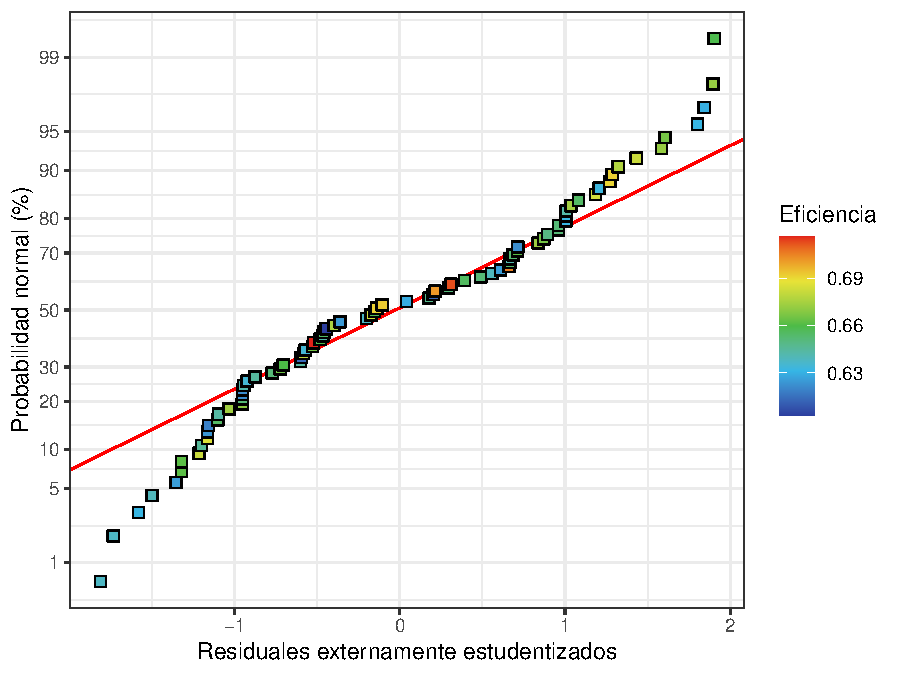
\includegraphics[width=\textwidth]{Articulo_Revista/Figs/fig9a_normal_residuales.pdf}\\
  {\small (a)}
\end{minipage}\hfill
\begin{minipage}[b]{0.49\textwidth}
  \centering
  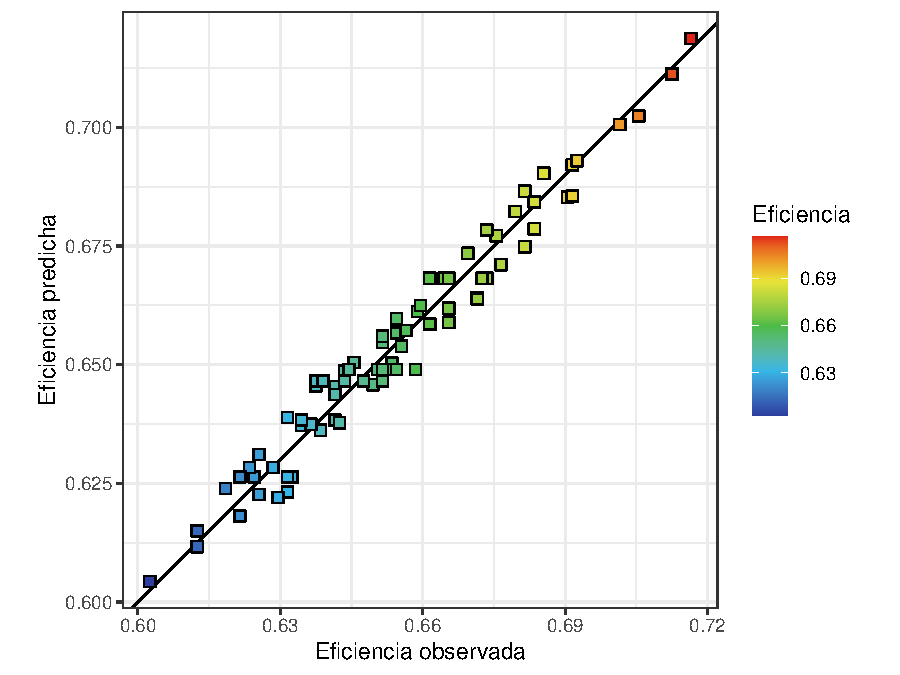
\includegraphics[width=\textwidth]{Articulo_Revista/Figs/fig9b_predicha_observada.pdf}\\
  {\small (b)}
\end{minipage}\\[6pt]
\begin{minipage}[b]{0.49\textwidth}
  \centering
  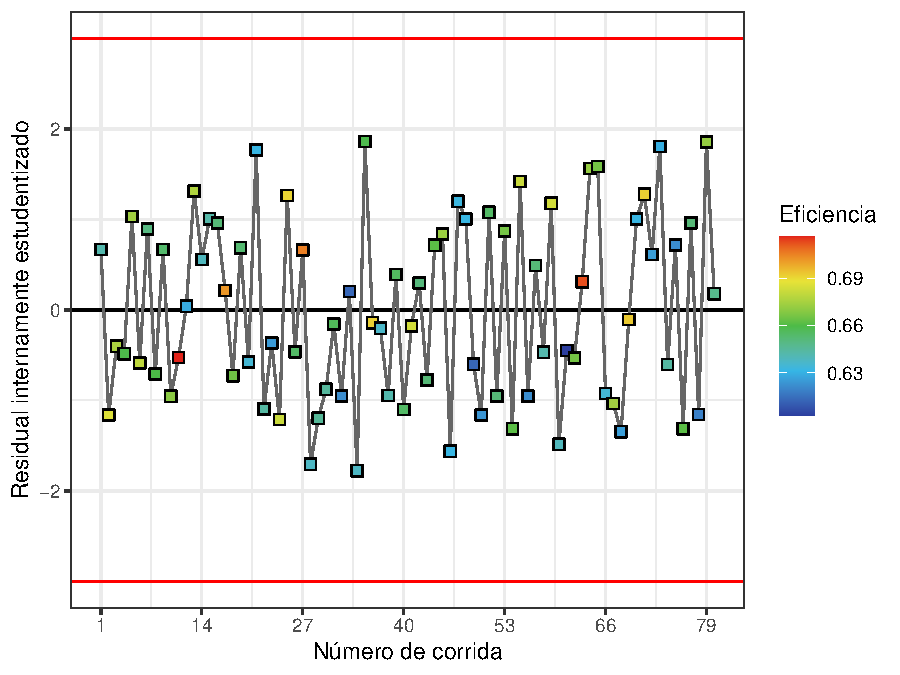
\includegraphics[width=\textwidth]{Articulo_Revista/Figs/fig9c_rint_corrida.pdf}\\
  {\small (c)}
\end{minipage}\hfill
\begin{minipage}[b]{0.49\textwidth}
  \centering
  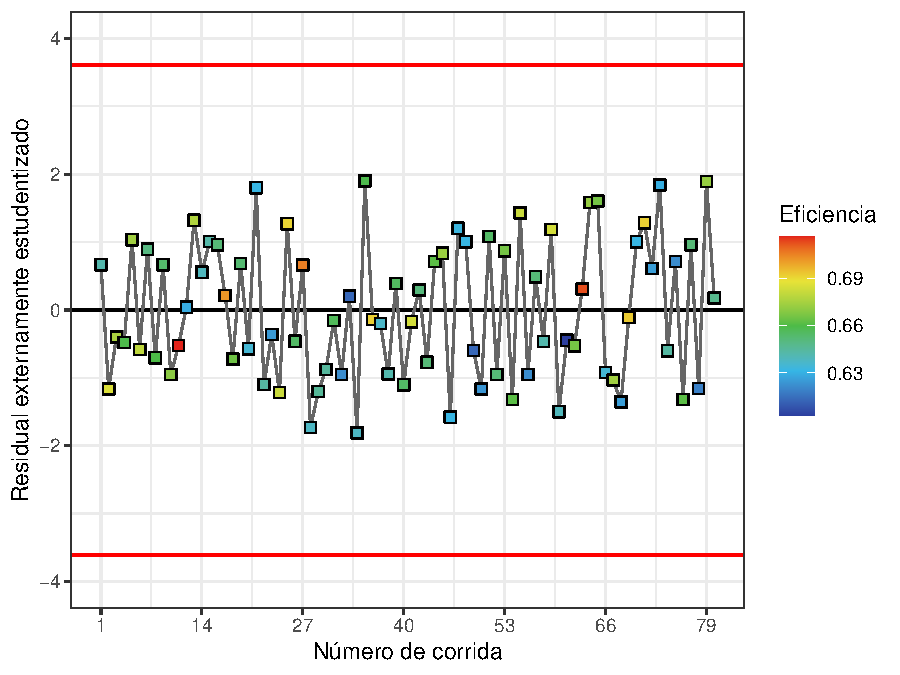
\includegraphics[width=\textwidth]{Articulo_Revista/Figs/fig9d_rext_corrida.pdf}\\
  {\small (d)}
\end{minipage}
\caption{Gráficos de diagnóstico: (a) probabilidad normal de los residuales externamente estudentizados, (b) eficiencia predicha frente a observada, (c) residuales internamente estudentizados y (d) residuales externamente estudentizados frente al número de corrida. Código: sección~10 de \texttt{mod\_lin.R}.}
\label{fig:diagnosticos}
\end{figure}

\begin{itemize}
  \item \textbf{(a) Probabilidad normal.} Cada residual se ubica frente al percentil que le correspondería si los residuales vinieran de una distribución normal; si la normalidad se cumple, los puntos quedan cerca de la recta. En la parte central los puntos siguen la recta. En los extremos se separan un poco y forman una S suave: los residuales más grandes en valor absoluto son menos extremos de lo que se esperaría con una normal, es decir, las colas son algo más livianas. La desviación es leve y no hay puntos aislados, así que el supuesto de normalidad es razonable.
  \item \textbf{(b) Predicha frente a observada.} Cada punto compara la eficiencia que predice el modelo con la que se midió. Si el modelo predice bien, los puntos quedan sobre la diagonal $y = x$. Aquí están muy cerca de ella en todo el rango, de 0.60 a 0.72, sin curvas ni zonas donde el modelo se equivoque de forma sistemática.
  \item \textbf{(c) Residuales internamente estudentizados frente al número de corrida.} Los puntos saltan de arriba abajo alrededor de cero, sin tendencia y sin que la dispersión crezca o se reduzca a lo largo de las corridas. Esto es compatible con errores independientes y de varianza constante. Todos están entre $-2$ y $2$, lejos de los límites de $\pm 3$ (líneas rojas) que usa Design Expert para señalar valores sospechosos.
  \item \textbf{(d) Residuales externamente estudentizados frente al número de corrida.} Las líneas rojas están en $\pm 3.61$. Ese límite es más amplio que $\pm 3$ porque tiene en cuenta que se revisan 80 corridas a la vez: con tantas corridas, alguna podría superar $\pm 3$ solo por azar (es el valor crítico $t$ con 60 grados de libertad y corrección de Bonferroni). Ninguna corrida lo supera, así que no hay observaciones atípicas.
\end{itemize}

En conjunto, los diagnósticos no muestran problemas con los supuestos del modelo.

\subsection{Superficies de respuesta}

Con el modelo ajustado se puede predecir la eficiencia en cualquier combinación de valores dentro de la región del experimento. La Figura~\ref{fig:contornos} muestra esas predicciones como gráficos de contorno, en función del ángulo y del diámetro, con la distancia fija en 50~mm y un panel para cada combinación de rodete y número de boquillas (sección~11 de \texttt{mod\_lin.R}). Se leen como un mapa topográfico: cada franja de color agrupa las combinaciones con la misma eficiencia predicha, las líneas negras separan franjas que difieren en 0.01 y los puntos rojos son las corridas del diseño con distancia de 50~mm. La Figura~\ref{fig:superficies} presenta las mismas predicciones como superficies en tres dimensiones, que reproducen la Figura~10 del artículo original.

\begin{figure}[ht]
\centering
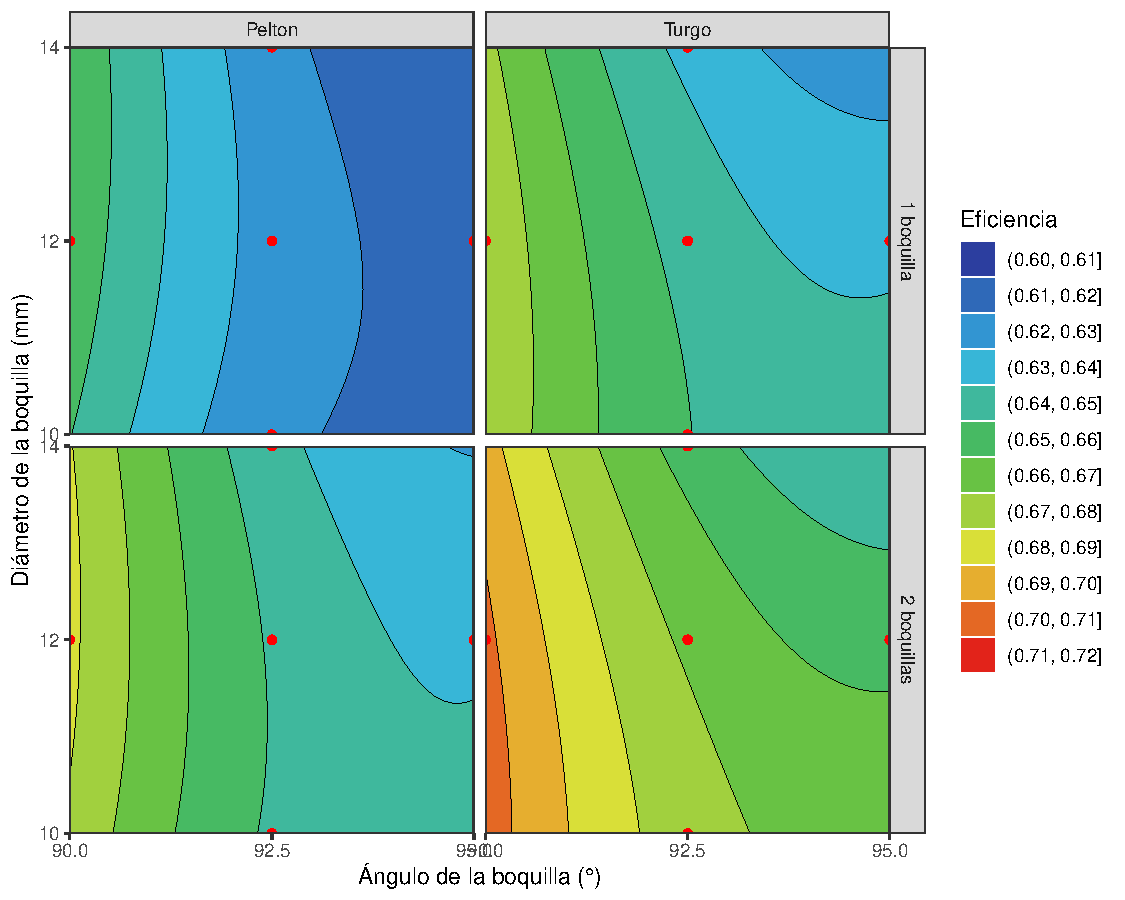
\includegraphics[width=0.8\textwidth]{Articulo_Revista/Figs/fig10_contornos.pdf}
\caption{Contornos de la eficiencia predicha según el ángulo y el diámetro de la boquilla, con la distancia en 50~mm, para cada tipo de rodete (columnas) y número de boquillas (filas). Código: sección~11 de \texttt{mod\_lin.R}.}
\label{fig:contornos}
\end{figure}

\begin{figure}[ht]
\centering
\begin{minipage}[b]{0.42\textwidth}
  \centering
  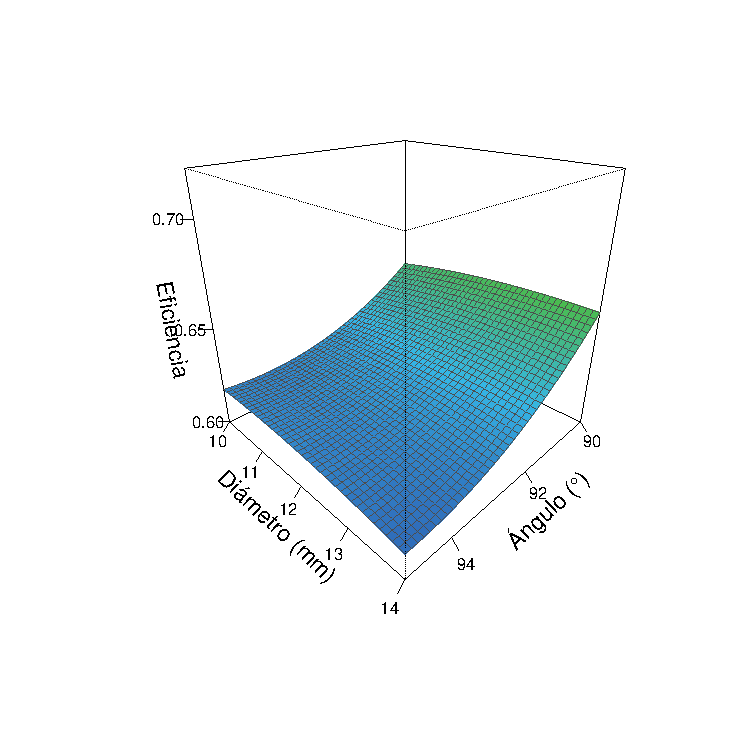
\includegraphics[width=\textwidth]{Articulo_Revista/Figs/fig10a_superficie_pelton_1.pdf}\\
  {\small (a) Pelton, 1 boquilla}
\end{minipage}\hspace{0.04\textwidth}
\begin{minipage}[b]{0.42\textwidth}
  \centering
  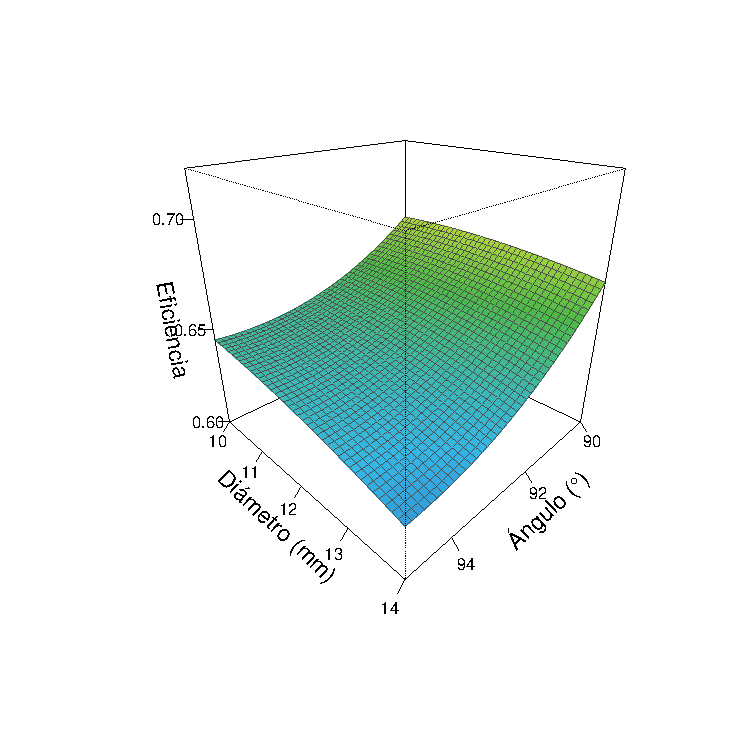
\includegraphics[width=\textwidth]{Articulo_Revista/Figs/fig10b_superficie_turgo_1.pdf}\\
  {\small (b) Turgo, 1 boquilla}
\end{minipage}\\[6pt]
\begin{minipage}[b]{0.42\textwidth}
  \centering
  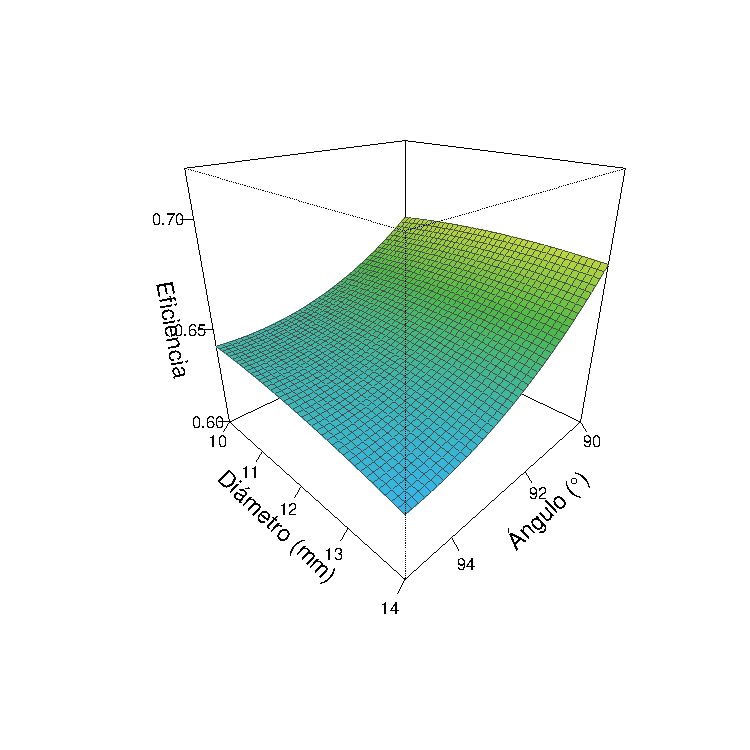
\includegraphics[width=\textwidth]{Articulo_Revista/Figs/fig10c_superficie_pelton_2.pdf}\\
  {\small (c) Pelton, 2 boquillas}
\end{minipage}\hspace{0.04\textwidth}
\begin{minipage}[b]{0.42\textwidth}
  \centering
  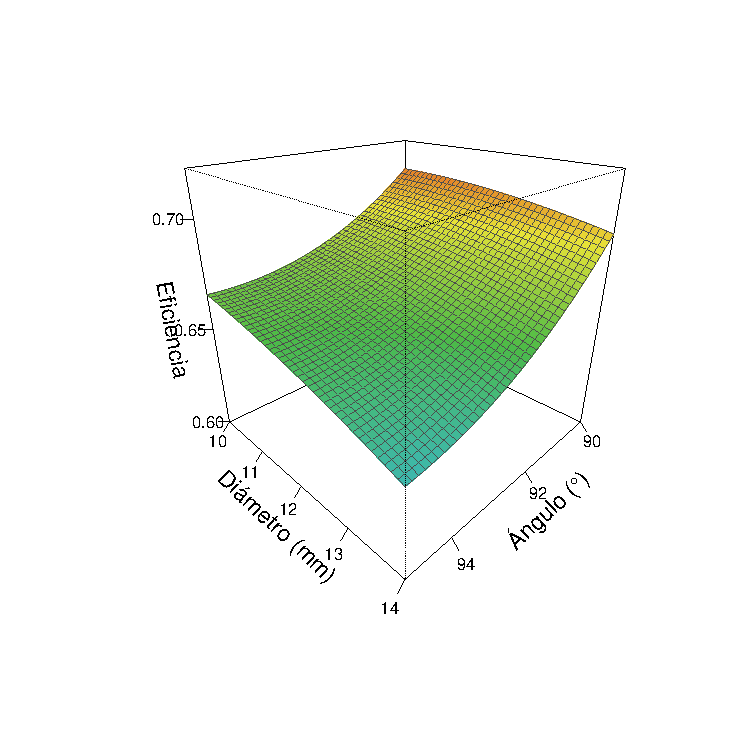
\includegraphics[width=\textwidth]{Articulo_Revista/Figs/fig10d_superficie_turgo_2.pdf}\\
  {\small (d) Turgo, 2 boquillas}
\end{minipage}
\caption{Superficies de respuesta de la eficiencia predicha según el ángulo y el diámetro de la boquilla, con la distancia en 50~mm. Código: sección~11 de \texttt{mod\_lin.R}.}
\label{fig:superficies}
\end{figure}

En los cuatro paneles la eficiencia predicha aumenta hacia la izquierda, es decir, hacia 90°, y las franjas son más angostas cerca de 90° que cerca de 95°: la eficiencia cambia rápido al alejarse de 90° y luego se estabiliza, que es el efecto del término cuadrático del ángulo. En el Pelton las franjas son casi verticales, lo que indica que el diámetro casi no cambia la eficiencia. En el Turgo las franjas se inclinan y la eficiencia es mayor con diámetros pequeños, sobre todo cerca de 95°, como lo indicaban las interacciones $BD$ y $AB$. Los paneles de abajo (dos boquillas) y los de la derecha (Turgo) alcanzan colores más altos, y la eficiencia predicha más alta de la figura está en el Turgo con dos boquillas, con 90° y diámetros pequeños.

\subsection{Condición de máxima eficiencia}

\citet{Lakdawala2025} reportan como condición óptima el rodete Turgo con dos boquillas, 95°, 14~mm y 40~mm, con una eficiencia predicha de 0.6619. El modelo replicado da la misma predicción en ese punto, y la corrida 53, hecha en esas condiciones, tuvo una eficiencia de 0.6655 (sección~12 de \texttt{mod\_lin.R}).

Sin embargo, ese no es el máximo del modelo. Al evaluar el modelo en una rejilla fina dentro de la región del experimento, la eficiencia predicha máxima de cada combinación de rodete y número de boquillas se alcanza siempre con 90° y 40~mm (Tabla~\ref{tab:maximos}). El máximo global es 0.7190, en el Turgo con dos boquillas, con 90°, 10.6~mm y 40~mm. Esto coincide con el análisis descriptivo, donde la eficiencia media más alta se dio con 90°, y con la corrida 11 (90°, 10~mm, 40~mm, Turgo con dos boquillas), que tuvo la mayor eficiencia observada, 0.7165. El artículo no detalla los criterios de su optimización, así que no es posible saber por qué su punto óptimo está en 95°.

\begin{table}[ht]
\centering
\caption{Condición de máxima eficiencia predicha dentro de la región del experimento para cada combinación de rodete y número de boquillas.}
\label{tab:maximos}
\begin{tabular}{llcccc}
\toprule
Rodete & Boquillas & Ángulo (°) & Diámetro (mm) & Distancia (mm) & Eficiencia predicha \\
\midrule
Pelton & 1 & 90 & 14.0 & 40 & 0.6711 \\
Pelton & 2 & 90 & 13.2 & 40 & 0.6935 \\
Turgo  & 1 & 90 & 11.6 & 40 & 0.6941 \\
Turgo  & 2 & 90 & 10.6 & 40 & 0.7190 \\
\bottomrule
\end{tabular}
\end{table}
